\documentclass[50pt]{article}
\usepackage[utf8]{inputenc}
\usepackage[spanish]{babel}
\usepackage[margin=2.5cm]{geometry}
\usepackage{amsmath,amssymb}
\usepackage{graphicx}
\usepackage{float}
\usepackage{enumitem}

\title{
    \vspace{-2.5cm} 
    {\centering 
\includegraphics[width=1.0\textwidth]{banner.png} \\[1cm]}
    \textbf{Coordenadas Polares y Cartesianas} \\[1cm]
    \large Taller de Investigación Pre-Cálculo: Dominando las Coordenadas Polares \\[4cm]
}  

\author{
    253110213 - Flores Soria Ximena \\
    253110012 - Alvarado Villegas Gael Salvador \\[4cm]
}

\date{Octubre, 2026}

\begin{document}
\maketitle
\begin{center}
    \vspace{1cm}
    
    \textbf{GRUPO:} TID-401 \\[0.8cm]
    
    \textbf{Docente:} Rubén Ramírez Gómez

\end{center}


\newpage
\section{Definición y Representación Gráfica}
 
\textbf{¿Qué es el Polo y qué es el Eje Polar?}
 
\begin{itemize}
  \item El \textbf{Polo} es el punto fijo central del sistema, equivalente al origen $(0,0)$ del sistema cartesiano.
  \item El \textbf{Eje Polar} es un semieje horizontal dirigido hacia la derecha desde el polo, equivalente al semieje positivo $x$.
\end{itemize}
 
\textbf{Dibuja un sistema de coordenadas polares y ubica los puntos}
$P_1\left(3,\frac{\pi}{4}\right)$, $P_2(2,\pi)$ y $P_3\left(4,\frac{3\pi}{2}\right)$.
 
\begin{figure}[H]
  \centering
  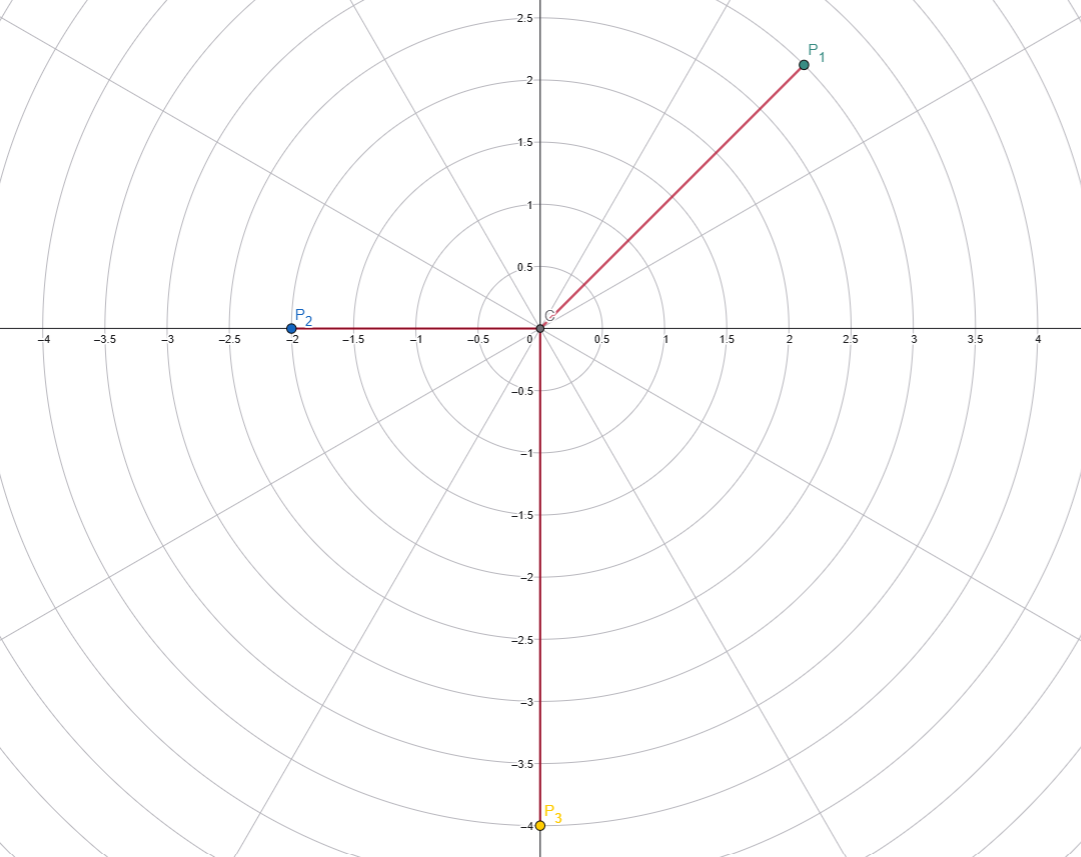
\includegraphics[width=0.6\textwidth]{coordPolares.png}
  \caption{Sistema de coordenadas polares.}
\end{figure}
 
\textbf{Reflexión:} En el plano cartesiano, cada punto $(x,y)$ es único. En polares, ¿puede un mismo punto tener más de un nombre?
 
Sí, puede tener infinitos nombres distintos ya que al dar una vuelta se le asigna un nombre, pero al dar una vuelta completa llegas al mismo lugar, al cual se le podría asignar otro nombre.
 

\section{El puente matemático (Conversiones)}
 
\textbf{Hacia Cartesianas:} Si conozco el radio ($r$) y el ángulo ($\theta$), ¿cómo obtengo $x$ e $y$?
 
Coseno se aplica sobre X y Seno sobre Y. Por lo tanto:
\[
\cos\theta=\frac{x}{r}\;\Rightarrow\; x=r\cos\theta,
\qquad
\sin\theta=\frac{y}{r}\;\Rightarrow\; y=r\sin\theta .
\]
 
\textbf{Hacia Polares:} Si conozco $(x,y)$, ¿cómo calculo la distancia al origen ($r$) y el ángulo ($\theta$)?
 
A través del teorema de Pitágoras y de la razón tangente
\[
r=\sqrt{x^2+y^2},
\qquad
\tan\theta=(\frac{y}{x}\;) \theta \Rightarrow\;\theta=\arctan\left(\frac{y}{x}\right).
\]
 
\textbf{Identidad clave:} ¿A qué es igual $x^2+y^2$ cuando se pasa a polares?
\[
x^2+y^2=(r\cos\theta)^2+(r\sin\theta)^2=r^2(\cos^2\theta+\sin^2\theta)=r^2
\quad\therefore\quad x^2+y^2=r^2 .
\]
 

\section{Visualización de Ecuaciones}
 
\textbf{¿Qué figura se forma con la ecuación $r=5$?}
 
Una circunferencia de radio 5 con centro en el polo, ya que todos los puntos están a distancia 5 del origen sin importar el ángulo.
 
\textbf{¿Qué figura se forma con la ecuación $\theta=\frac{\pi}{4}$?}
 
Una línea recta que pasa por el origen y que aumenta 4 en $x$ por 1 en $y$ 
 
\textbf{¿Qué sucede con la expresión $\dfrac{x^2+y^2}{x^2}$ al convertirla totalmente a polares?}
\[
\frac{x^2+y^2}{x^2}=\frac{r^2}{(r\cos\theta)^2}=\frac{r^2}{r^2\cos^2\theta}=\frac{1}{\cos^2\theta}=\sec^2\theta .
\]

 

\section{El concepto de ``Límite al Origen''}
 
No depende del ángulo $\theta$ , ya que no importa la dirección o trayectoria por la que se aproxima. r debe ser independiente de $\theta$ ya que si no se cumple esto el límite no existe.
 

\newpage
\section{Formulario}
 
\subsection*{Diagrama de un punto $(r,\theta)$}
 
\begin{figure}[H]
  \centering
  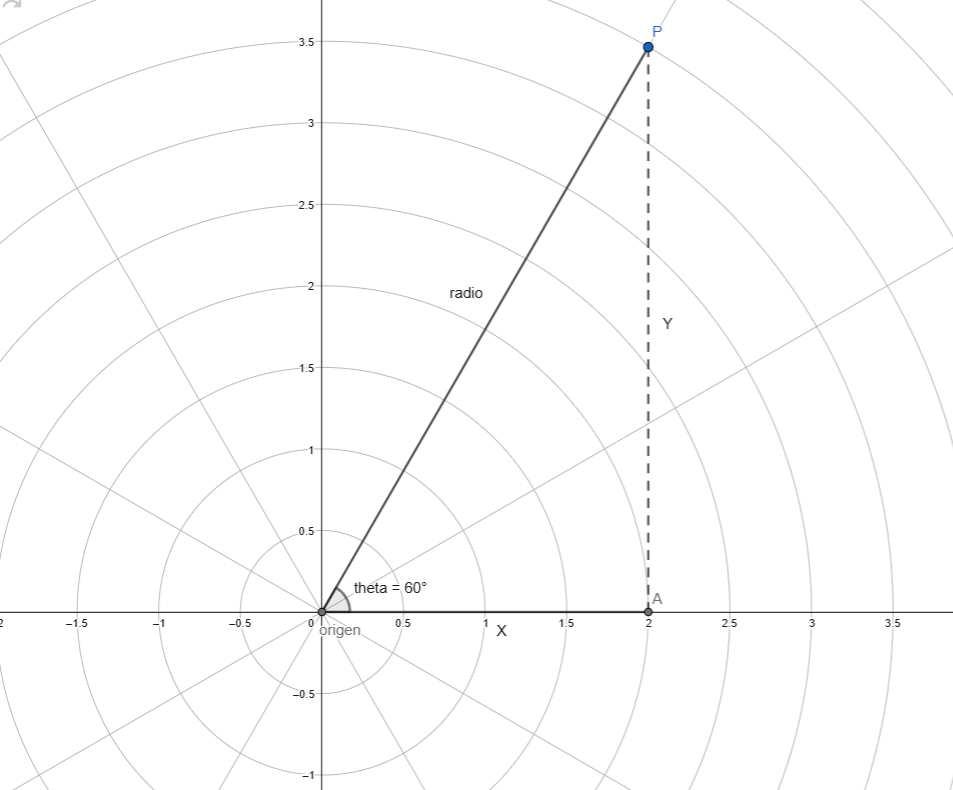
\includegraphics[width=0.50\textwidth]{diag2pto.png}
  \caption{Diagrama de un punto $\left(4,\frac{\pi}{3}\right)$.}
\end{figure}
 
\subsection*{Fórmulas de conversión}
 
\begin{table}[H]
  \centering
  \begin{tabular}{|c|c|}
    \hline
    Polares a cartesianas & Cartesianas a polares \\
    \hline
    $x=r\cos\theta$ & $r=\sqrt{x^2+y^2}$ \\
    \hline
    $y=r\sin\theta$ & $\theta=\arctan\left(\dfrac{y}{x}\right)$ \\
    \hline
  \end{tabular}
  \caption{Fórmulas de conversión.}
\end{table}
 
\subsection*{Identidad pitagórica trigonométrica}
\[
\sin^2\theta+\cos^2\theta=1,
\qquad
x^2+y^2=r^2 .
\]
 
\subsection*{Tabla de valores de $\sin$ y $\cos$}
 
\begin{table}[H]
  \centering
  \begin{tabular}{|c|c|c|c|}
    \hline
    Ángulo ($\theta$) & Radianes\\
    \hline
    $0^\circ$   & $0$\\
    \hline
    $90^\circ$  & $\dfrac{\pi}{2}$\\
    \hline
    $180^\circ$ & $\pi$\\
    \hline
    $270^\circ$ & $\dfrac{3\pi}{2}$\\
    \hline
  \end{tabular}
  \caption{Valores de seno y coseno.}
\end{table}
 

\newpage
\section{Ejercicios: Cartesianas a Polares}
 

 
\subsection*{1. El Clásico de la Raíz}
\[
f(x,y)=\sqrt{x^2+y^2}=\sqrt{r^2}=r
\]
\[
\boxed{f=r}
\]
 
\subsection*{2. La Trampa de las Potencias Diferentes}
\[
f(x,y)=\frac{x^2}{x^2+y^2}=\frac{(r\cos\theta)^2}{r^2}=\frac{r^2\cos^2\theta}{r^2}=\cos^2\theta
\]
\[
\boxed{f=\cos^2\theta}
\]

 
\subsection*{3. El Exponente Negativo o Fraccionario}
\[
f(x,y)=e^{-(x^2+y^2)}=e^{-r^2}
\]
\[
\boxed{f=e^{-r^2}}
\]

 
\subsection*{4. La Mezcla de Grados (Homogeneidad)}
\[
f(x,y)=\frac{xy}{\sqrt{x^2+y^2}}=\frac{(r\cos\theta)(r\sin\theta)}{\sqrt{r^2}}=\frac{r^2\cos\theta\sin\theta}{r}=r\cos\theta\sin\theta
\]
\[
\boxed{f=r\cos\theta\sin\theta}
\]
.
 
\subsection*{5. Ejercicios Falso / Verdadero}
 
\begin{enumerate}
  \item ``Si $(x,y)\to(0,0)$, entonces $r\to0$ independientemente de cuánto valga $\theta$.''
 
  \textbf{Verdadero.} Como $r=\sqrt{x^2+y^2}$ es la distancia al origen, acercarse al origen equivale a que $r\to0$, sin importar la dirección $\theta$ de aproximación.
 
  \item ``La expresión $x^2+y^2$ en polares es igual a $r$.''
 
  \textbf{Falso.} Es igual a $r^2$, pues $x^2+y^2=r^2(\cos^2\theta+\sin^2\theta)=r^2$. Es $\sqrt{x^2+y^2}$ la que es igual a $r$.
 
  \item ``Si al convertir un límite a polares el resultado final contiene a $\theta$ (por ejemplo: $\cos\theta$), el límite no existe.''
 
  \textbf{Falso.} Si $\theta$ aparece en una expresión acotada que se multiplica por un factor que tiende a $0$, el límite sí existe. Por ejemplo, $\lim_{r\to0} r\cos\theta\sin\theta=0$ (ejercicio 4). El límite solo deja de existir cuando, después de hacer $r\to0$, el resultado final todavía depende de $\theta$ (como en el ejercicio 2, donde queda $\cos^2\theta$).
\end{enumerate}
 

\section{Ejercicios: Polares a Cartesianas}
 
 
\subsection*{1. Puntos en los Ejes (Nivel Básico)}
 
\textbf{Punto A:} $(5,\pi)$
\[
x=5\cos\pi=5(-1)=-5,\qquad y=5\sin\pi=5(0)=0
\]
\[
\boxed{A=(-5,\,0)}
\]
 
\textbf{Punto B:} $\left(3,\dfrac{\pi}{2}\right)$
\[
x=3\cos\frac{\pi}{2}=3(0)=0,\qquad y=3\sin\frac{\pi}{2}=3(1)=3
\]
\[
\boxed{B=(0,\,3)}
\]
 
\subsection*{2. Puntos en Cuadrantes (Uso de Trigonometría)}
 
\textbf{Punto C:} $\left(4,\dfrac{\pi}{4}\right)$
\[
x=4\cos\frac{\pi}{4}=4\cdot\frac{\sqrt2}{2}=2\sqrt2,\qquad
y=4\sin\frac{\pi}{4}=4\cdot\frac{\sqrt2}{2}=2\sqrt2
\]
\[
\boxed{C=\left(2\sqrt2,\,2\sqrt2\right)\approx(2.83,\,2.83)}
\]
 
\textbf{Punto D:} $\left(2,\dfrac{2\pi}{3}\right)$
\[
x=2\cos\frac{2\pi}{3}=2\left(-\frac12\right)=-1,\qquad
y=2\sin\frac{2\pi}{3}=2\cdot\frac{\sqrt3}{2}=\sqrt3
\]
\[
\boxed{D=\left(-1,\,\sqrt3\right)\approx(-1,\,1.73)}
\]
 
\subsection*{3. La Identidad Inversa}
 
\textbf{Ecuación:} $r=4\cos\theta$
 
Se multiplican ambos lados por $r$ y se sustituye $r^2=x^2+y^2$ y $r\cos\theta=x$:
\[
r^2=4r\cos\theta\;\Rightarrow\;x^2+y^2=4x
\]
Completando el cuadrado:
\[
x^2-4x+y^2=0\;\Rightarrow\;(x-2)^2+y^2=4
\]
\[
\boxed{(x-2)^2+y^2=4}
\]

 
\subsection*{4. La Recta Polar}
 
\textbf{Ecuación:} $r\sin\theta=2$
 
Como $y=r\sin\theta$:
\[
\boxed{y=2}
\]
Es una recta horizontal que pasa por $(0,2)$.
 
\subsection*{5. La Secante}
 
\textbf{Ecuación:} $r=\dfrac{3}{\cos\theta}$
 
Se multiplica por $\cos\theta$ y se usa $x=r\cos\theta$:
\[
r\cos\theta=3\;\Rightarrow\;\boxed{x=3}
\]
Es una recta vertical que pasa por $(3,0)$.
 
\end{document}
 